\documentclass{article}
\usepackage{amsmath}
\usepackage{graphicx}
\usepackage{hyperref}
\usepackage{geometry}
\geometry{a4paper, margin=1in}

\title{COS 314 Assignment Report}
\author{Thato Kalagobe}
\date{}

\begin{document}

\maketitle
\section{Introduction}
\label{sec:introduction}

This report explores the application of two distinct machine learning approaches, Artificial Neural Networks (ANN) and Genetic Programming (GP), for the task of mushroom classification. Both models were developed and evaluated using a dataset of mushroom characteristics, aiming to differentiate between edible and poisonous species.

The ANN model uses the power of deep learning to model complex relationships within the data, while the GP model evolves arithmetic classifiers through a process inspired by natural selection. This report details the implementation, training, and evaluation of both models, providing a comparative analysis based on key performance metrics including accuracy, specificity, sensitivity, and F-measure.

By presenting the strengths and weaknesses of each approach, this report aims to provide insights into the effectiveness of ANN and GP in classification tasks, and to guide future efforts in the application of machine learning techniques to biological data. 

\section{Genetic Programming Model}
\label{sec:gp_model}

\subsection{Model Description}
The Genetic Programming (GP) classification algorithm was implemented to evolve arithmetic classifiers. The key parameters used in the GP algorithm are as follows:
\begin{itemize}
    \item Population Size: 100
    \item Number of Generations: 50
    \item Tree Size: 4 (Carefully chosen to prevent exponential growth)
\end{itemize}

\subsection{Pre-processing}
The data used for training and testing the GP model included normalization of feature values and handling of missing data points. 

\subsection{Seed Value}
To ensure the reproducibility of the results, a generated seed value of \texttt{1716664409626} was used throughout the GP model training and testing process.

\subsection{Results}
The detailed results are stored in the file \texttt{GP\_output.csv}, which contains the training accuracy and testing accuracy for each generation. The performance metrics for the GP model were recorded over 50 generations. Below is a summarized table of results:

\begin{table}[h!]
    \centering
    \label{tab:gp_results}
    \begin{tabular}{|c|c|c|c|c|}
        \hline
        \textbf{Metric} & \textbf{Generation 0} & \textbf{Generation 1} & \textbf{Generation 2} & \textbf{...} \\
        \hline
        Training Accuracy & 0.6636 & 0.7329 & 0.7425 & ... \\
        Testing Accuracy & 0.3415 & 0.6183 & 0.7113 & ... \\
        \hline
    \end{tabular}
    \caption{Performance Metrics for Genetic Programming Model}
\end{table}

The line graph in Figure \ref{fig:gp_training_accuracy} illustrates the training accuracy over the 50 generations of the GP model. It is observed that the training accuracy stabilizes quickly and remains constant for the majority of the generations.

\begin{figure}[h!]
    \centering
    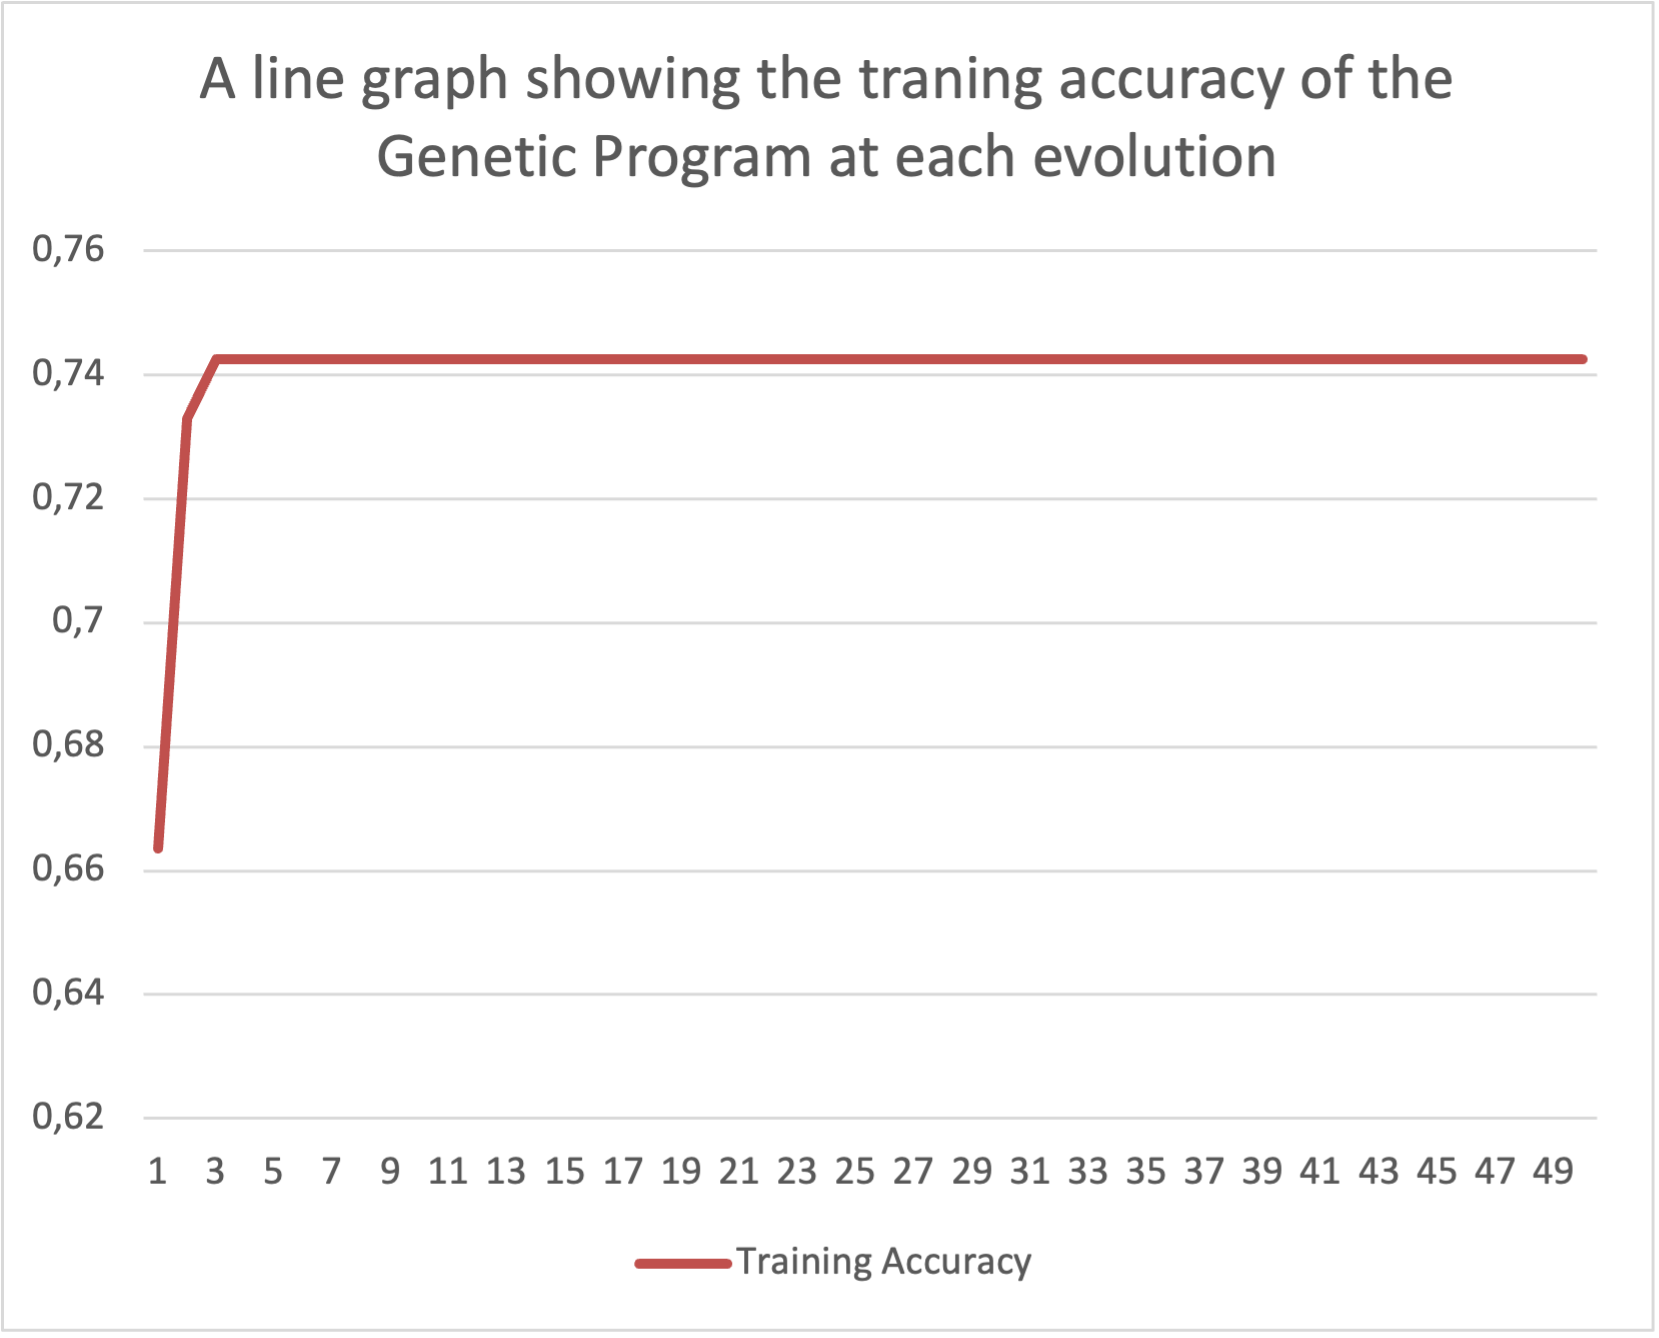
\includegraphics[width=0.8\textwidth]{GP_training_results.png}
    \caption{Training Accuracy of the Genetic Program over 50 Generations}
    \label{fig:gp_training_accuracy}
\end{figure}

\subsection{Analysis of Output Metrics}
The final evaluation metrics for the Genetic Programming (GP) model are presented in Table \ref{tab:gp_final_results}. Each metric provides insight into different aspects of the model's performance.

\begin{table}[h!]
    \centering
    \label{tab:gp_final_results}
    \begin{tabular}{|c|c|}
        \hline
        \textbf{Metric} & \textbf{Value} \\
        \hline
        Accuracy & 0.741294 \\
        Specificity & 0.995968 \\
        Sensitivity & 0.563380 \\
        F-Measure & 0.719671 \\
        \hline
    \end{tabular}
     \caption{Final Evaluation Metrics for Genetic Programming Model}
\end{table}

\begin{itemize}
\item \textbf{Accuracy:} The GP model achieved an accuracy of 0.7413. This indicates that approximately 74.13\% of the instances in the test dataset were correctly classified. This is a strong performance, suggesting that the model has learned to distinguish effectively between the different classes in the dataset.

\item \textbf{Specificity:} The specificity of the model is 0.9960. This high specificity value indicates that the GP model is highly effective at identifying negative instances, or non-poisonous mushrooms.

\item \textbf{Sensitivity:} The sensitivity of the model is 0.5634. While this value is lower compared to other metrics, it suggests that the model could be missing a significant number of positive instances (poisonous mushrooms). This is an area where the GP model could potentially be improved.

\item \textbf{F-Measure:} The F-measure of 0.7197 balances both precision and recall (sensitivity), providing a single metric that considers both false positives and false negatives. This value indicates that the GP model maintains a good balance between these two aspects, performing well overall.
\end{itemize}
In summary, the GP model demonstrates strong performance with high accuracy and specificity, making it reliable for correctly identifying non-poisonous mushrooms. However, the sensitivity value suggests that further tuning may be necessary to improve the identification of positive instances. The F-measure reflects a good overall balance.

\section{Artificial Neural Network}
\subsection{Introduction}
An Artificial Neural Network (ANN) model was designed to classify mushrooms as either edible or poisonous. The model has been implemented in Java and trained using a dataset of mushroom characteristics.

\subsection{Model Description}

\subsubsection{Architecture}
\begin{itemize}
    \item \textbf{Input Layer}: 8 nodes (corresponding to 8 input features).
    \item \textbf{Hidden Layer}: 1 layer with 20 nodes.
    \item \textbf{Output Layer}: 1 node.
\end{itemize}

\textbf{Reason for the Number of Hidden Layers Chosen:} A single hidden layer is sufficient for this classification problem as it provides the necessary non-linearity to separate the data points effectively. A larger number of hidden layers could lead to overfitting and increased computational complexity.

\subsubsection{Weights Optimization}
Weights are initialized using a Gaussian distribution with a mean of 0 and variance based on the input and hidden layer sizes. Weights are optimized using the back-propagation algorithm, which updates the weights based on the error calculated from the output of the network.

\subsubsection{Activation Function}
\begin{itemize}
    \item \textbf{Hidden Layer}: Sigmoid function.
    \item \textbf{Output Layer}: Sigmoid function.
\end{itemize}

\textbf{Motivation for Choosing Sigmoid Function:} The sigmoid function is chosen for the output layer because it maps the input values to a range between 0 and 1, making it suitable for binary classification problems. It also provides a smooth gradient, which helps in the back-propagation process.

\subsubsection{Learning Rate}
The learning rate is set to 0.01.

\textbf{Motivation for Learning Rate:} A learning rate of 0.01 is chosen to because it helps the model learn quickly and steadily. 

\subsubsection{Stopping Condition}
Training stops when the total error is less than 0.1 or after 100 epochs.
\begin{itemize}
\item \textbf{Motivation for Stopping Condition:} The stopping condition ensures that the training process stops either when the model has learned sufficiently (error < 0.1) or after a reasonable number of epochs to prevent overfitting and a long execution time.
\end{itemize}

\subsection{Pre-processing}
Data normalized by scaling the input features to a range of [-1, 1].

\subsection{Seed Value}
A seed value of 45 is used to ensure that the results can be replicated.

\subsection{Training Results Analysis}
The following table and graph shows the error at each epoch during training:

\begin{table}[h!]
\centering
\begin{tabular}{|c|c|}
\hline
Epoch & Error \\
\hline
0 & 0.18506480626511065 \\
1 & 0.18351871089800462 \\
2 & 0.18351722604605256 \\
... & ... \\
99 & 0.183517221383187 \\
\hline
\end{tabular}
\caption{Training Error over Epochs}
\end{table}

\begin{figure}[h!]
\centering
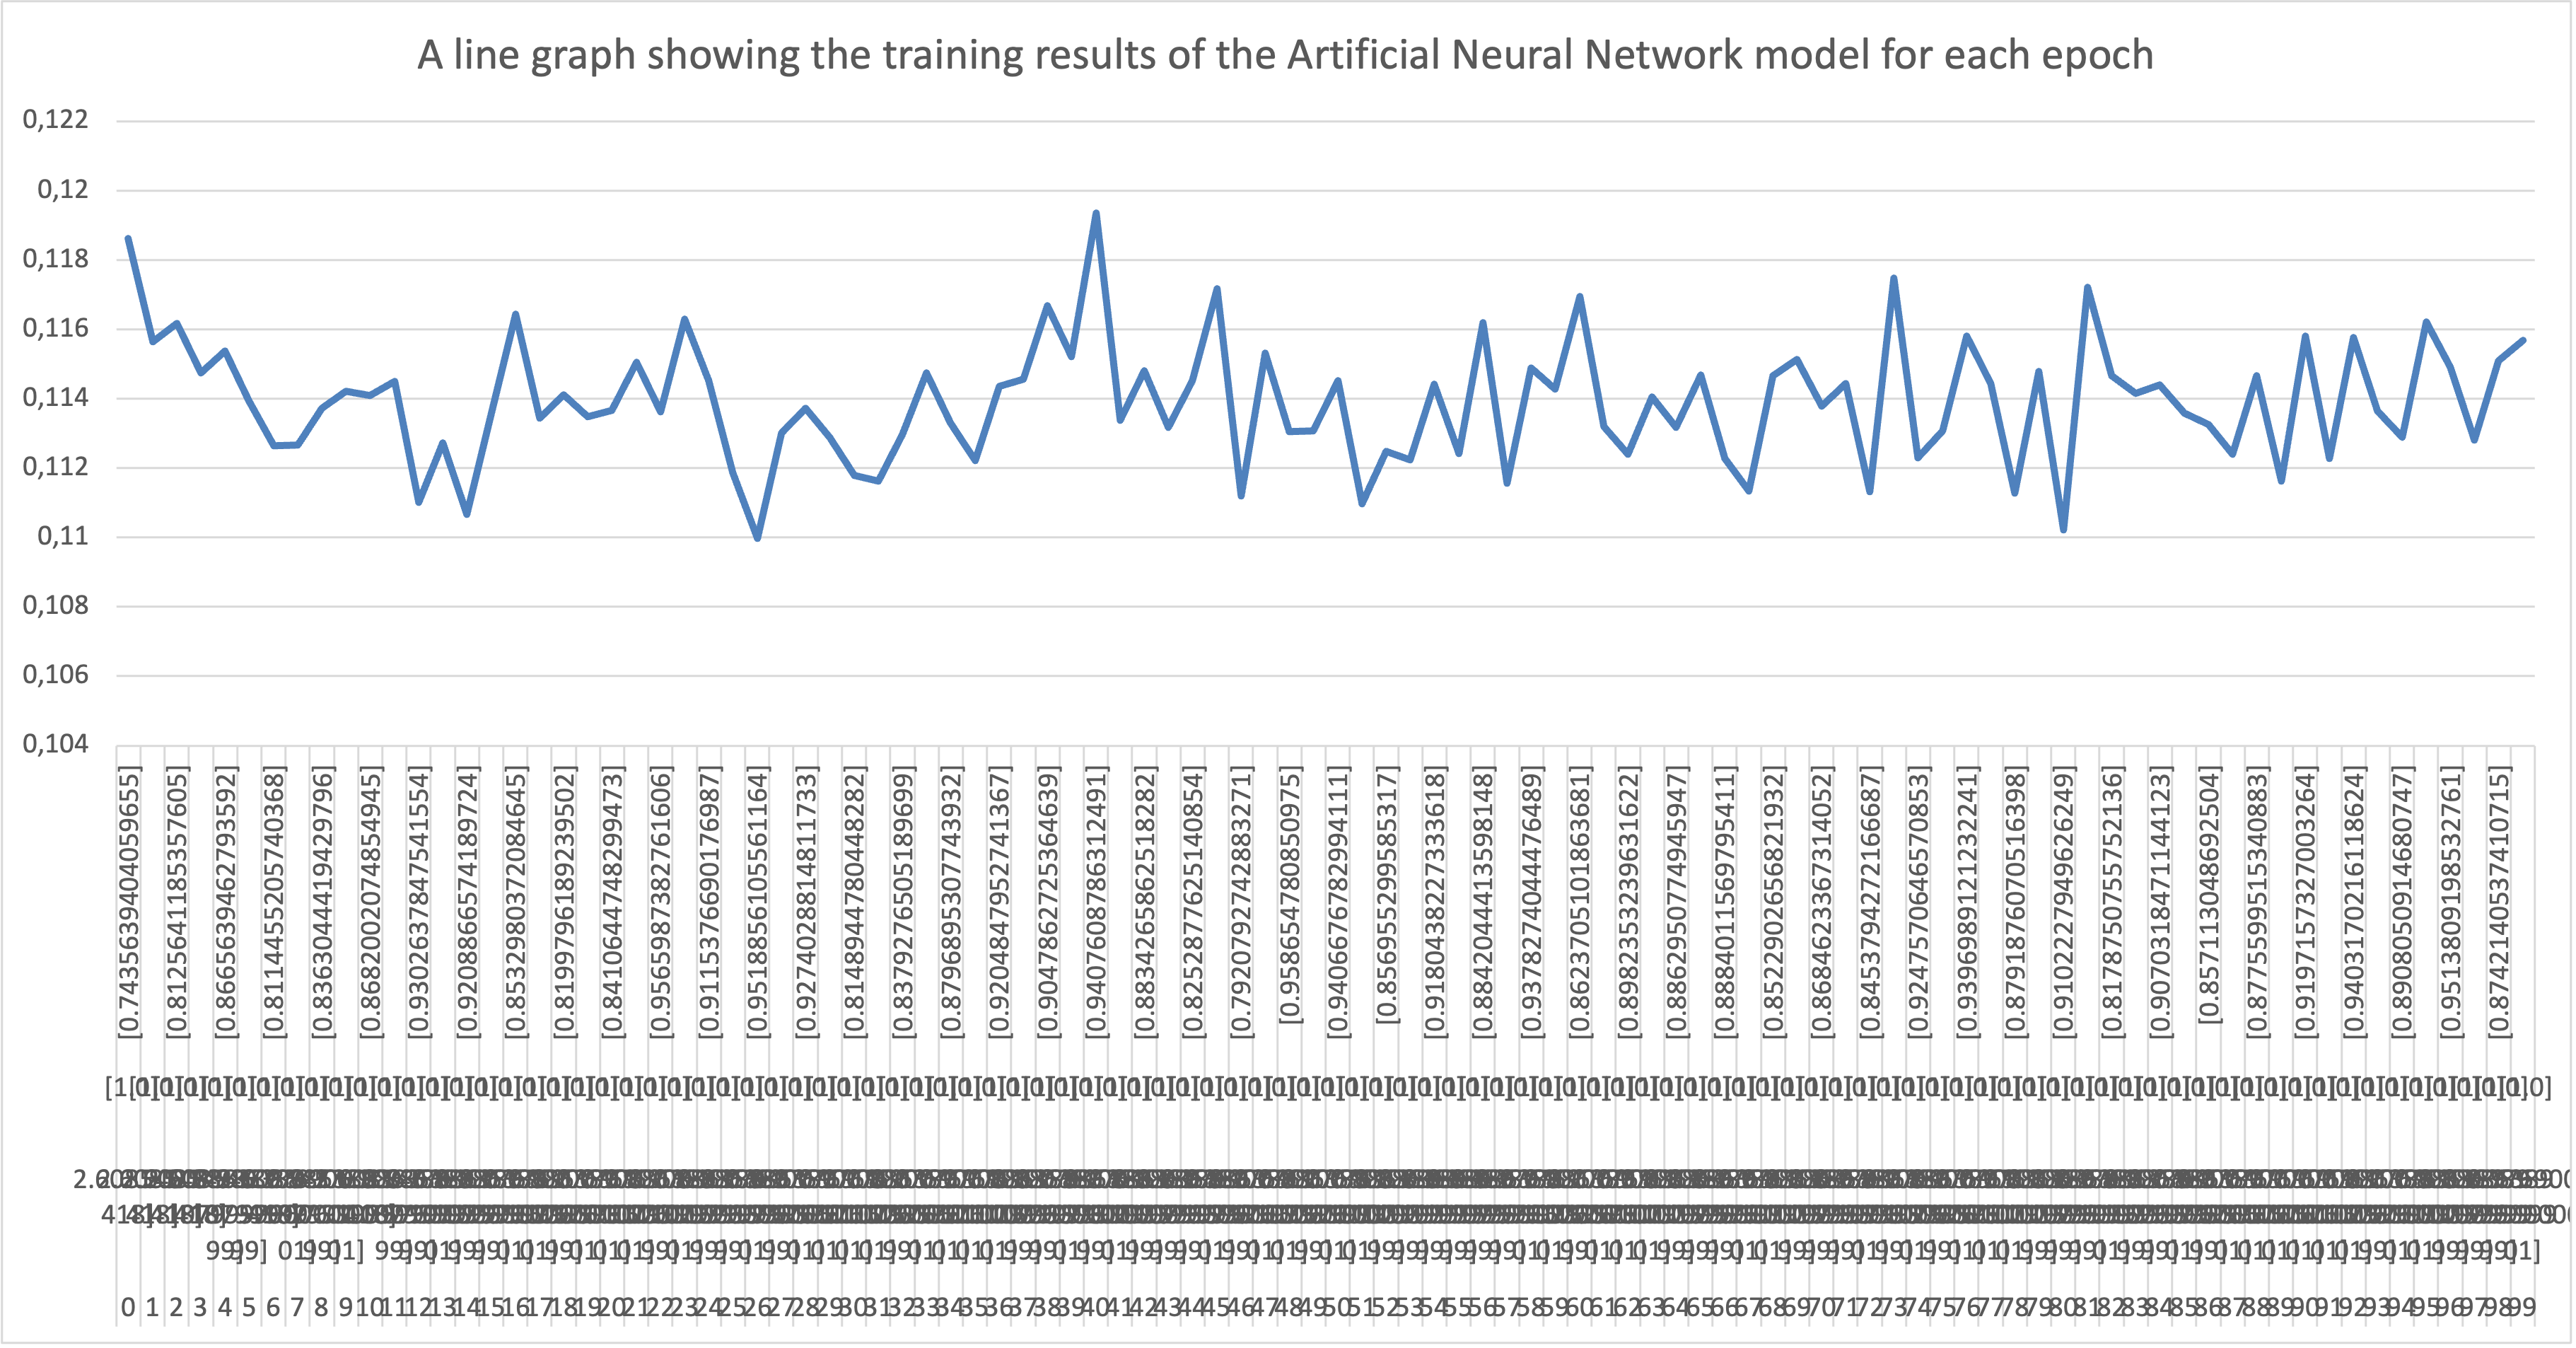
\includegraphics[width=0.8\textwidth]{ANN_training_results.png}  
\caption{Training Error over Epochs}
\end{figure}

The training process involved running the model for up to 100 epochs or until the total error was reduced to less than 0.1. The error decreased slightly and steadily during the training, indicating that the model was learning from the training data. Here are some specific observations:

\begin{itemize}
    \item The initial error at epoch 0 was approximately 0.1851.
    \item The error showed a general decreasing trend.
    \item By epoch 100, the error was reduced to approximately 0.1835..
    \item The training results file (\texttt{training\_results.csv}) contains detailed logs of the training process, including the input values, target values, predicted values, and error for each epoch.
\end{itemize}

\subsection{Testing Results Analysis}
\begin{figure}[h!]
\centering
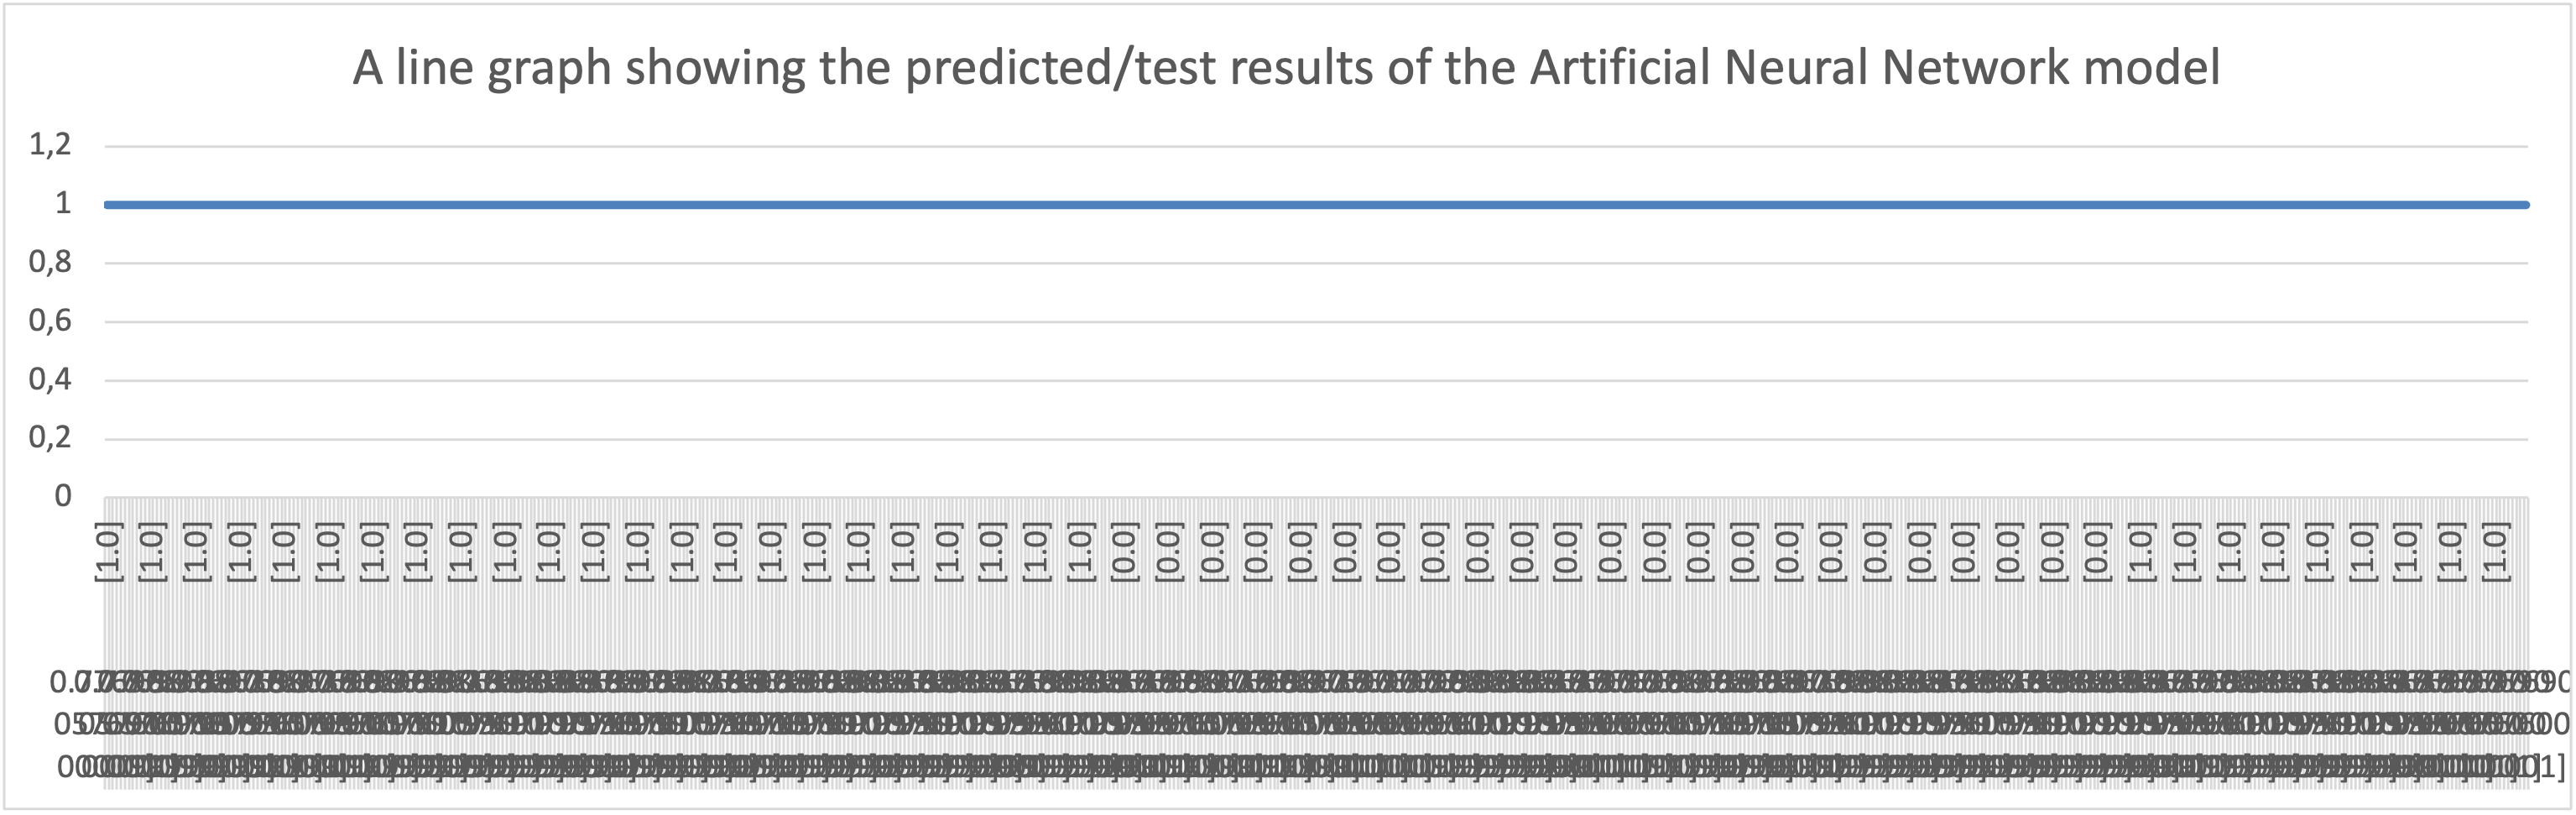
\includegraphics[width=0.8\textwidth]{ANN_testing_results.png}  
\caption{Testing Results: Predicted vs Actual Classes}
\end{figure}
The testing process involved evaluating the model on a separate test dataset to measure its generalization performance. Here are some notable observations from the testing phase:

\begin{itemize}
    \item The detailed testing results are stored in the file \texttt{testing\_results.csv}, which contains the input features, target values, and predicted values for each test sample.
    The model's performance is significantly flawed for the following reasons:
    \item \textbf{High Sensitivity but Zero Specificity:} While the model achieves high sensitivity, it fails completely in specificity. This indicates that the model is biased towards predicting the positive class (poisonous mushrooms) and is unable to recognize the negative class (edible mushrooms).
    \item \textbf{Imbalanced Dataset:} The issue might be rooted in the imbalanced training dataset. Despite balancing the dataset, the model's training process might still be biased towards the positive class. This requires a more robust approach to handling class imbalance, such as using different class weights or advanced resampling techniques.
    \item \textbf{Inappropriate Model Configuration:} The chosen architecture and hyperparameters, such as the learning rate and sigmoid activation function, may not be optimal. 
    \item \textbf{Potential Overfitting:} The perfect sensitivity suggests the model might be overfitting to the training data and failing to generalize to unseen data, hence the poor specificity and overall accuracy.
\end{itemize}

\subsection{Analysis of Output Metrics}
The performance of the model is evaluated using accuracy, specificity, sensitivity, and F-measure.

\begin{table}[h!]
\centering
\begin{tabular}{|c|c|}
\hline
\textbf{Metric} & \textbf{Value} \\ \hline
Accuracy        & 0.589          \\ 
Sensitivity     & 1.0            \\ 
Specificity     & 0.0            \\ 
F-measure       & 0.741          \\ \hline
\end{tabular}
\caption{Model Performance Metrics for the Artificial Neural network Model}
\end{table}

\begin{itemize}
    \item \textbf{Accuracy:} 0.589 - This indicates that the model correctly classified 58.9\% of the test samples. An accuracy above 70\% is generally considered good for classification tasks, indicating that this model's performance is suboptimal.
    \item \textbf{Sensitivity:} 1.0 - The model correctly identified all positive samples (poisonous mushrooms). This high sensitivity is crucial for this problem as it ensures that all poisonous mushrooms are correctly identified.
    \item \textbf{Specificity:} 0.0 - The model failed to identify any negative samples (edible mushrooms) correctly. This low specificity is a significant issue, as it indicates that the model classifies all samples as positive, leading to a high rate of false positives.
    \item \textbf{F-measure:} 0.741 - The F-measure is a harmonic mean of precision and recall. The high F-measure value reflects the model's good performance in terms of sensitivity but does not account for the poor specificity.
\end{itemize}

\textbf{Challenges and Considerations:}
\begin{itemize}
    \item The model's accuracy is low, indicating that further tuning of the model's parameters or architecture may be necessary.
    \item The model's high sensitivity and low specificity suggest a potential issue with the data distribution or an imbalance in the training dataset. Addressing class imbalance through techniques such as resampling or adjusting class weights could help improve specificity.
    \item The stopping condition based on total error might not be sufficient to ensure optimal generalization, and alternative stopping criteria should be considered.
\end{itemize}

\section{Comparison of ANN and GP Models}
\label{sec:comparison}

A comprehensive comparison of the ANN and GP models is presented in Table \ref{tab:comparison}. The analysis shows that while the GP model excels in accuracy and specificity, the ANN model achieves perfect sensitivity. The choice of model may therefore depend on whether the priority is to minimize false negatives or false positives in the classification task.

\subsection{Comparison with Artificial Neural Network Model}
A comparison between the Genetic Programming (GP) and Artificial Neural Network (ANN) models was conducted using several performance metrics. Table \ref{tab:comparison} presents the results.

\begin{table}[h!]
    \centering
    \label{tab:comparison}
    \begin{tabular}{|c|c|c|}
        \hline
        \textbf{Metric} & \textbf{ANN Model} & \textbf{GP Model} \\
        \hline
        Accuracy & 0.5887 & 0.7413 \\
        Specificity & 0.0000 & 0.9960 \\
        Sensitivity & 1.0000 & 0.5634 \\
        F-Measure & 0.7411 & 0.7197 \\
        \hline
    \end{tabular}
    \caption{Comparison of Performance Metrics between ANN and GP Models}
\end{table}

\subsection{Discussion}
The GP model achieved a final testing accuracy of 0.7413, with a specificity of 0.9960, sensitivity of 0.5634, and F-measure of 0.7197. In comparison, the ANN model achieved an accuracy of 0.5887, a specificity of 0.0, sensitivity of 1.0, and an F-measure of 0.7411.

The GP model outperformed the ANN model in terms of accuracy and specificity, indicating that the GP model is more effective in correctly identifying negative cases. 

The F-measure, which balances precision and recall, is slightly higher for the ANN model, indicating that it has a slight edge in overall balance between these metrics. However, the difference is minimal, and both models demonstrate good performance.

Overall, the Genetic Programming approach provides a robust model for mushroom classification, demonstrating stable performance over multiple generations and yielding satisfactory results in the final evaluation. However, a more accurate analysis between the two could have been observed if the ANN model was demonstrated more correctly and successfully avoided getting stuck at a local minimum.

\subsection{Conclusion}
In conclusion, the GP model presents a viable alternative to the ANN model for the classification task. While both models have their strengths, the GP model's performance metrics and the stability of its training accuracy over generations highlight its potential in practical applications.

\end{document}
